% !TEX root = ../Robotik.tex

\chapter{Software-Architekturen für mobile Robotersysteme}
\begin{displayquote}
	Unter einem Roboter verstehen wir eine frei programmierbare Maschine, die auf
	Basis von Umgebungssensordaten in geschlossener Regelung in Umgebungen
	agiert, die zur Zeit der Programmierung nicht genau bekannt und/oder
	dynamisch und oder nicht vollständig erfassbar sind. \\
	-- \textit{Joachim Herzberg, Mobile Roboter}
\end{displayquote}

\section{Probleme und Anforderungen}
\subsection{Umgebung mobiler Roboter}
Bei \textbf{mobilen Robotern} ist die Umgebung im Detail \textbf{nicht bekannt
und generell nicht kontrollierbar}. Alle Aktionen sind \textbf{von der aktuellen
Umgebung abhängig} und \textbf{Details sind nur während der Ausführung} der
Aktion bekannt.

Mobile Roboter müssen in einer geschlossen Regelung:
\begin{enumerate}
	\item Erfassung der Umgebung mit Sensoren
	\item Auswertung der Daten
	\item Planung der Aktionen
	\item Umsetzung der Aktionen mittels Koordination der Aktuatoren
\end{enumerate}

\subsection{Roboterkontroll-Architekturen}
\subsubsection{Herausforderungen}
Robotersysteme bestehen im allgemeinen aus den Gebieten \textbf{Wahrnehmung},
\textbf{Planung} und \textbf{Handlung}. Die Herausforderungen die hierdurch
entstehen sind:
\begin{itemize}
	\item Erfassung und Auswertung der Sensorwerte
	\item Planung der Pfade
	\item Vermeidung von Hindernissen
	\item Ausführung komplexer Algorithmen in langen Zeitzyklen
\end{itemize}

\subsubsection{Probleme bei der Software-Erstellung zur Roboterkontrolle}
Roboter sind \textbf{eingebettete Systeme}, die in einem geschlossenen
Regelkreis die Sensorströme in \textbf{Echtzeit verarbeiten}. Dadurch entstehen
diese Probleme:

\begin{itemize}
	\item Untschiedliche Aufgaben $\Rightarrow$ Unterschiedliche Zeitzyklen
	\item Unterschiedlicher Zeitskalen $\Rightarrow$ Abbildung des Kontroll-
		und Datenflusses in der Architektur ist nicht standardisiert
	\item Für etliche algorithmische Teilprobleme sind \textbf{keine effizienten
		Verfahren} bekannt
	\item \textbf{Prozessorkapazität ist begrenzt}
\end{itemize}

\subsection{Anforderungen an das Kontrollsystem eines autonomen Roboters}

\begin{description}
	\item[Robustheit]
		Die Umgebung des Systems kann sich ständig ändern. Auf diese muss der
		Roboter sinnvoll reagieren, obwohl die verwendeten Modelle der Umgebung
		ungenau ist.
	\item[Unterschiedliche Ziele]
		Roboter verfolgt zu einem Zeitpunkt eventuell in Konflikt stehende Ziele.
		z.B.: Ziel ansteuern und Hinterniss ausweichen
	\item[Sensorwerte von mehreren Sensoren]
		Sensordaten können verrauscht sein und damit fehlerhafte und inkonsiste
		Messwerte liefern. z.B. außerhalb seines Bereichs und dies nicht überprüfen
		kann.
	\item[Erweiterbarkeit]
		Bei neuen Sensoren, sollte diese leicht in das Programm integriert werden
		können.
\end{description}

\section{Mögliche Modelle}

\subsection{Klassisches Modell - der funktionale Ansatz}

{
\begin{wrapfigure}{r}{0.4\textwidth}
	\centering
	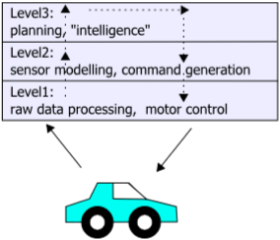
\includegraphics[width=0.39\textwidth]{Resources/PNG/ClassicModell.png}
	\caption{Oben nach unten: Planer, Navigator, Pilot}
\end{wrapfigure}

Das \textbf{klassische Model} wird auch als hierarchisches Model oder
funktionales Model bezeichnet. Ist ein Top-Down Ansatz, besteht aus drei
Abstraktionsebenen.

Dieses Model hat unterschiedliche Namen:
\begin{itemize}
	\item Sense-Think-Act-Cycle (STAC)
	\item Sense-Model-Plan-Act (SMPA)
\end{itemize}

\begin{description}
	\item[Sense:] \small Vorverarbeitung der Daten
	\item[Model:] \small Konstruktion oder Aktualisierung eines Weltmodells
	\item[Plan:] \small Alle Entscheidungen basieren auf dem Weltmodell
	\item[Act:] \small Ausführung der Aktionen und Befehle
\end{description}

Zyklus wird ständig wiederholt $\Rightarrow$ wenn alle Ebenen richtig
funktionieren resultiert daraus ein intelligentes Verhalten und die Erfüllung
der Aufgabe.

}

\paragraph{Nachteile:}
\begin{itemize}
	\item \textbf{Sequentieller Ansatz} $\Rightarrow$ \textbf{lange
		Kontrollzykluszeit}
	\item \textbf{Gesamtsystem anfällig} $\Rightarrow$ Modulfehler führt zum
		scheitern des Gesamtsystems
	\item Weltmodell muss alle zur Planung notwendigen Informationen enthalten
	\item Planer hat nur Zugriff auf das Weltmodell $\Rightarrow$ Während Planung
		kann sich Umwelt verändert haben
\end{itemize}

\subsection{Verhaltensbasiertes Modell}
\paragraph{Grundlegender Gedanke} Intelligentes Verhalten wird nicht durch
komplexe, monolithische Kontrollstrukturen erzeugt, sondern durch das
Zusammenführen der richtigen einfachen Verhalten und deren Interaktion.

\paragraph{Definition}
\begin{itemize}
	\item Engere Verbindung zwischen \textbf{Wahrnehmung} und \textbf{Aktion}
	\item Jede \textbf{Roboterfunktionalität} wird in einem \textbf{Behavior}
		gekapselt
	\item Alle \textbf{Behaviors} werden \textbf{parallel ausgeführt}
	\item Jedes Behavior Modul operiert unabhängig von den anderen
	\item Alle Behaviors können auf alle Fahrzeugsensoren zugreifen und
		gewissermaßen die Aktuatoren ansteuern.
\end{itemize}

\subsection{Hybrider Ansatz}
{
\begin{wrapfigure}{r}{0.4\textwidth}
	\includegraphics[width=0.4\textwidth]{Resources/PDF/HybridModel}
	\caption{Schema des Hybridmodell}
\end{wrapfigure}

Nutzt die Vorteile der \textbf{Subsumption Architektur} und der \textbf{SMPA-
Architektur}. Der verhaltensbasierte Anteil ist nicht geeignet, auf längere
Sicht zielgerichtet Aktionen zu koordinieren $\Rightarrow$ SMPA-Anteil

Die \textbf{Handlungsplanung} arbeitet auf hoher, strategischer Stufe
in langen Zeitzyklen.

Die \textbf{mittlere Kontrollebene} hat die taktische Aufga\-be, die jeweils
\textbf{nächste Aktion aus dem Plan aus\-zusuchen}, zu instanzieren und auf die
Ebene der Verhaltensbausteine zu zerlegen. Des weiteren muss die die
Rückmeldung von der Aktionsüberwachung interpretieren und entscheiden ob eine
Aktion erfolgreich abgeschlossen ist. $\Rightarrow$ entscheiden, ob die
Handlungsplanung einen anderen Plan erstellen muss.

Die \textbf{reaktive Aktionsüberwachung} enthält die Verhaltensbausteine auf
operativer Ebene, die in schellen Zeitzyklen die physische Roboteraktion
anstoßen und überwachen

}

\paragraph{Kritik}
\begin{itemize}
	\item Mittlere Komponente benötigt den größten konzeptuellen und programmiertechnischen Auf\-wand
	\item Das mittlere Teilproblem ist deutlich komplexer als die beiden anderen
\end{itemize}

\subsection{Probabilistische Robotik}
Berücksichtigung der \textbf{Unsicherheit der Wahrnehmung und der Aktionen}.

\textbf{Schlüsselidee:} Information in Form von Wahrscheinlichkeitsdichten
repräsentieren. Eine \textbf{Lokalisie\-rung} der Roboter wird unter Verwendung
von Wahrscheinlichkeitstheorie oder einer Wahrscheinlichkeitsverteilung eine
Aussage über die Umgebung treffen.

\textbf{Probabilistische Wahrnehmung:} wenn man Sensorwerte schätzen kann,
dann kann man mit Wahrscheinlichkeitstheorie eine Aussage über die Umgebung
treffen.

\textbf{Probabilistisches Handeln:} aufgrund der Unsicherheit über die
Umgebung ist auch das Handeln mit Unsicherheit behaftet. Mit probabilistischen
Ansätzen besteht die Möglichkeit Entscheidungen trotz Unsicherheit zu treffen.

\textbf{Vorteil:} probabilistische Verfahren können auch mit weniger
präzisen Umgebungsmodellen angewandt werden.

\textbf{Nachteil:} weniger effizient wegen komplexer Berechnungen,
Approximation erforderlich

\subsection{Subsumption-Architektur in Bezug auf die Anforderungen des
Roboter\-steuer\-ungssystems}

\paragraph{Robustheit:} Wenn einige Steuerungsmodule ausfallen, arbeiten bei der Subsumption-Architektur die restlichen Schichten einwandfrei $\Rightarrow$ \textbf{eingeschränktes, aber sinnvolles Verhalten möglich}

\paragraph{Unterschiedliche Ziele}
\begin{itemize}
	\item Mehrere Teilsituationen können verschiedene Verhaltenselemente sinvoll
		machen, die sich widersprechen können.
	\item Die Wichtigkeit einer Handlung hängt vom Kontext ab, d.h. höhere Ziele
		können niederere Ziele ersetzen.
	\item Alle zu einem Zeitpunkt möglichen Verhaltenselemente werden parallel
		bearbeitet.
	\item Das \textbf{resultierende Verhalten wird in Abhängigkeit von
		Umwelteinflüssen dynamisch} bestimmt
	\item Das Gesamtergebnis hängt nicht von einer übergeordneten Instanz ab
\end{itemize}

\paragraph{Sensorwerte von mehreren Sensoren}
\begin{itemize}
	\item Der Roboter muss auch bei inkonsistenten Informationen eine
		Entscheidung fällen
	\item Die Subsumption-Architektur sieht keine zentrale Verarbeitung und
		Speichung der Umweltdaten vor
	\item Jedes Modul reagiert nur auf die Daten einzelner Sensoren, es muss
		\textbf{kein konsistentes Abbild der Umwelt erschaffen werden}
\end{itemize}

\paragraph{Erweiterbarkeit} Das bestehende Verhalten kann jederzeit durch
Hinzufügen weiterer Schichten um komplexere Funktionen erweitert werden

\section{Robot Operating System (ROS)}
ROS bietet einene Standard für Roboterkontrollsoftware. \textbf{DAS
Architekturschema für Roboterkontrollsoftware} gibt es nicht $\Rightarrow$
Unterstützung der Softwareentwicklung durch Middleware wie ROS.

\textbf{Zweck}: soll die Entwicklung von Software für Roboter vereinfachen und wiederkehrende Aufgaben standardisieren

\begin{figure}[H]
	\begin{center}
		\includegraphics[scale=0.6]{Resources/PDF/FileSystem}
		\caption{Filesystem, das ROS zugrunde liegt}
		\label{fig:PDF/FileSystem}
	\end{center}
\end{figure}

\subsection{Design Prinzipien}
In ROS kommunizieren die verschiedenen Nodes über den Master, dabei können
die verschiedenen Nodes und der Master auf verschiedenen Rechnern laufen.
Einzige Bedingung ist, dass die Nodes den Master erreichen können.

\begin{description}
	\item[Master] Dient zur Koordinierung und Kommunikation von Nodes. Er ist
		damit der wichtigste Knoten. Er bietet eine Serviceregistry für synchrone
		Kommunikation zwischen Nodes und ist Message Broker für asynchronen
		Nachrichtenaustausch.
	\item[Node] Wird in ROS as Package publiziert. Ein Node muss sich beim Master
		registieren und kann über ihn mit anderen Nodes kommunizieren. Ein Node
		ist in ROS ein Process mit einer bestimmten Funktionalität. Ist ein Node
		fehlerhaft hat dies in der Regel wenig Auswirkungen auf andere Nodes.
\end{description}

\subsubsection{Parameter Server und Konfigurationsdateien}
Der Parameter Server auf dem Master enthält \textbf{eine Art Wörterbuch für
Werte}. Alle Ressourcen wie Nodes, Messages oder Parameter existieren darin in
einer hierachischen Namensstruktur. In ihm werden z.B.: die
Konfigurationsdateien gespeichert.

\subsection{Asynchrone Kommunikation}
Der asynchrone Nachrichtenaustausch funktioniert über das
\textbf{Publish-Subscribe} Pattern. Hierbei kann ein Node kann entweder
Nachrichten an den Master  publiziere, dafür benutzt er ein bestimmtes Topic.
Er kann jedoch auch verschiedene Topics abbonieren um Nachrichten zu empfangen
sobald diese publiziert werden. Ein Node hat dabei kein Limit an Topics die er
nutzen kann. Ein Topic ist hierbei ein einfacher String. Die Kommunikation
findet dabei über TCP/IP Socket stat.

\begin{verbatim}
 Node2                                                           Master
   |                      register publisher                       |
   |--------------------- topic: "farbsensor" -------------------> |
                                                                   |
 Node1                                                             |
   |                          subscribe                            |
   |--------------------- topic: "farbsensor" -------------------> |
                                                                   |
 Node2                                                             |
   |                           publish                             |
   |-- topic: "farbsensor" message: { r: 0.1, g: 0.1, b: 0.1 } --> |
                                                                   |
 Node1                                                             |
   |<- topic: "farbsensor" message: { r: 0.1, g: 0.1, b: 0.1 } --- |
\end{verbatim}

Die Nachrichten (\textbf{Messages}) die dabei übertragen werden können sind
streng typisiert. Eine Message kann \textbf{andere Messages, oder Felder von
Messages} enthalten. Die möglichen Datentypen sind hierbei die primitiven Typen
\textbf{int, float und bool}.

\subsection{Sychrone Kommunikation}
Die synchrone Kommunikation wird durch Services gelöst. Ein Node kann beim
Master einen Service registrieren. Ein zweiter Node kann daraufhin einen
Request schicken und erhält von der entsprechenen Node eine Response. Dies ist
besonders geeignet für RMI und einmalige Anfragen.

\begin{verbatim}
 Node1                                                           Master
   |                      register service                         |
   |------------------- service: "farbsensor" -------------------> |
                                                                   |
 Node2                                                             |
   |                        call service                           |
   |------------------------- getfarbe --------------------------> |
                                                                   |
 Node1                                                             |
   |<------------------------ getfarbe --------------------------- |
   |----------------- { r: 0.1, g: 0.1, b: 0.1 } ----------------> |
                                                                   |
 Node2                                                             |
   |                          response                             |
   |<---------------- { r: 0.1, g: 0.1, b: 0.1 } ----------------- |
\end{verbatim}
